\documentclass{article}
\usepackage{tikz}
\usetikzlibrary{positioning}
\usetikzlibrary{shapes.geometric}
\usetikzlibrary{shapes.callouts}
\pagestyle{empty}

\newcommand{\win}[1]{
  \begin{scope}[shift={#1}]
    \begin{scope}[scale=0.25]
      \draw [very thick,draw=green!50!black,fill=green]
            (0,0) .. controls (1.5,-0.5) and (1,-2.0) .. (0,-3)
                  .. controls (0.25, -2) and (-2, -1.5) .. (0,0);
      \draw [thin] (0,0) .. controls (0,-1) and (0.5,-2) .. (0,-3);
    \end{scope}
  \end{scope}}
 
\newcommand{\loss}[1]{
  \begin{scope}[shift={#1}]
    \begin{scope}[scale=0.25]
      \draw [very thick,draw=brown,fill=yellow!50!brown]
            (0,0) .. controls (-1.0,-0.5) and (-0.35,-2.0) .. (0,-3)
                  .. controls (-1.25, -1.75) and (1, -1.5) .. (0,0);
      \draw [thin] (0,0) .. controls (0,-1) and (-0.75,-2) .. (0,-3);
    \end{scope}
  \end{scope}}
  

\begin{document}

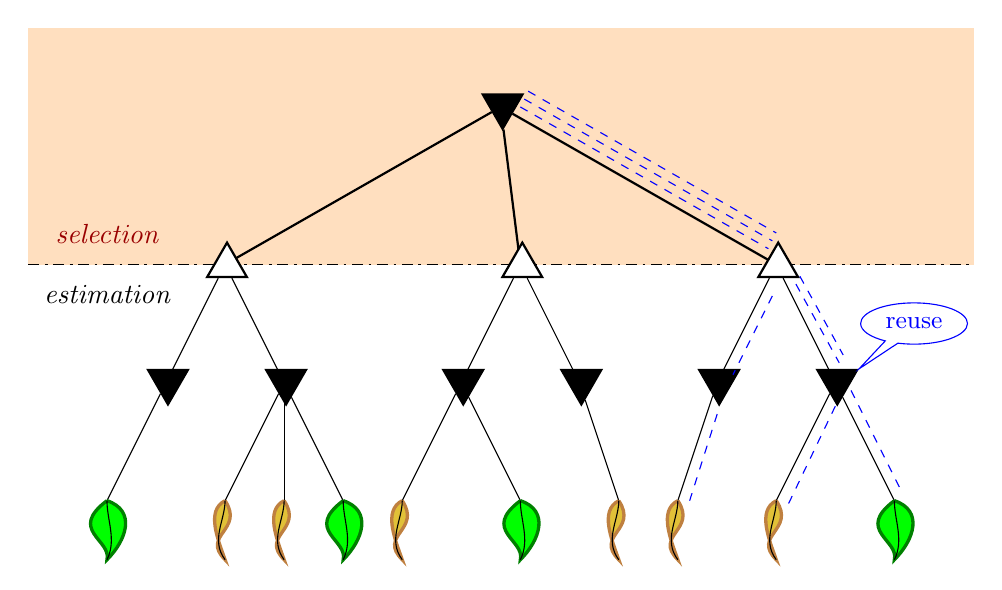
\begin{tikzpicture}
[node/.style={shape=isosceles triangle,isosceles triangle apex angle=60,
  thick},
black/.style={node,draw,fill=black,thick,rotate=30},
white/.style={node,draw,fill=white,thick,rotate=-30},
win/.style={node,shape=kite,draw=green!50!white,fill=green,below},
loss/.style={node,shape=kite,
            kite upper vertex angle=45,
            kite lower vertex angle=90,
            scale=0.75,
            draw=brown!50!black,fill=brown,below},
sample/.style={draw,thin,blue,dashed},
boundary/.style={dash pattern=on 4pt off 2pt on 1pt off 2pt}]

\draw [draw,fill,orange!25!white] (-6.0,1.0) rectangle (6.0,-2.0);
\draw[boundary] (-6.0,-2.0) -- (6.0,-2.0)
    (-5.0,-2.0) node [above=4pt,red!60!black] {\it selection}
    (-5.0,-2.0) node [below=4pt] {\it estimation};

\draw (0,0) node (root) [black] {};

\draw [thick] (root) -- ++(3.5,-2.0)
	node (s1) [white] {};
\draw [] (s1) -- ++( 0.75,-1.5)
	node (s11) [black] {}
        +(1.0,0.75) node [ellipse callout, callout absolute
        pointer={(s11.east)},draw,blue] {{\small reuse}};

\draw [] (s1) -- ++( -0.75,-1.5)
        node (s12) [black] {};
\draw [] (s11) -- ++( 0.75,-1.5)
        node (s111) {}; \win {(s111)};
\draw [] (s11) -- ++( -0.75,-1.5)
        node (s112) {}; \loss {(s112)};
\draw [] (s12) -- ++( -0.5,-1.5)
        node (s121) {}; \loss {(s121)};

\draw [thick] (root) -- ++(0.25,-2.0)
	node (s2) [white] {};
\draw [] (s2) -- ++( 0.75,-1.5)
	node (s21) [black] {};
\draw (s2) -- ++( -0.75, -1.5)
	node (s22) [black] {};
\draw [] (s21) -- ++( +0.5,-1.5)
	node (s211) {}; \loss {(s211)};
\draw (s22) -- ++( 0.75,-1.5)
	node (s221) {}; \win {(s221)};
\draw [] (s22) -- ++( -0.75,-1.5)
	node (s222) {}; \loss{(s222)};

\draw [thick] (root) -- ++(-3.5,-2.0)
	node (s3) [white] {};
\draw (s3) -- ++( 0.75,-1.5)
	node (s31) [black] {};
\draw [] (s3) -- ++( -0.75,-1.5)
	node (s32) [black] {};
\draw (s31) -- ++( 0.75,-1.5)
	node (s311) {}; \win {(s311)};
\draw [] (s31) -- ++( 0,-1.5)
	node (s312) {}; \loss {(s312)};
\draw  (s31) -- ++( -0.75,-1.5)
	node (s313) {}; \loss {(s313)};
\draw  [] (s32) -- ++( -0.75,-1.5)
	node (s321) {}; \win {(s321)};

% samples
\draw [sample] (0,0) ++(0.25,0.0) -- ++(3.15, -1.8)
                        ++(0.35,-0.45) -- ++(0.55, -1.0)
                        ++(-0.05,-0.55) -- ++(-0.6, -1.25);
\draw [sample] (0,0) ++(0.3,0.1) -- ++(3.15, -1.8)
                        ++(0.35,-0.45) -- ++(0.55, -1.0)
                        ++(0.1,-0.45) -- ++(0.65, -1.3);
\draw [sample] (0,0) ++(0.35,0.2)  -- ++(3.15, -1.8)
                     ++(-0.05, -0.8) -- ++(-0.5, -1.0)
                     ++(-0.2, -0.5) -- ++(-0.35, -1.1);
\end{tikzpicture}
\end{document}
